\documentclass[11pt, twoside, pdftex]{article}

% This include all the settings that we should use for the document
\newcommand{\PDFTitle}{SignalTap with Verilog Designs}
\newcommand{\commonPath}{../../../Common}
\newcommand{\datePublished}{Mar 2022}

\newcommand{\versnum}{21.1} %version number quartus/AMP
\newcommand{\quartusname}{Quartus\textsuperscript{\textregistered} Prime}	
\newcommand{\textBar}{For \quartusname{} \versnum{}}
\newcommand{\thisyear}{2022 } %for copyright
\newcommand{\company}{FPGAcademy.org}
\newcommand{\longteamname}{FPGAcademy.org}
\newcommand{\teamname}{FPGAcademy}
\newcommand{\website}{FPGAcademy.org}

\newcommand{\productAcronym}{AMP}
\newcommand{\productNameShort}{Monitor Program}

\newcommand{\productNameMedTM}{Monitor Program}
\newcommand{\productNameMed}{Monitor Program}

%\newcommand{\headerLogoFilePath}[1]{#1/FPGAcademy.png}



\setlength\topmargin{-0.25in}
\setlength\headheight{0in}
\setlength\headsep{0.35in}
\setlength\textheight{8.5in}
\setlength\textwidth{7in}
\setlength\oddsidemargin{-0.25in}
\setlength\evensidemargin{-0.25in}
\setlength\parindent{0.25in}
\setlength\parskip{0in} 

\pdfpagewidth 8.5in
\pdfpageheight 11in

% listings is a package that supports encapsulating source code in LaTeX conveniently

\usepackage{listings}
% add support for graphics
\usepackage{graphicx}
\usepackage[usenames, dvipsnames]{color}

\def\expandparam\lstinputlisting[#1]#2{\edef\tmp{\noexpand\lstinputlisting[#1]{#2}}\tmp}

\widowpenalty 10000
\clubpenalty 10000

%%%%%%%%%%%%%%%%%%%% Source Code Formatting %%%%%%%%%%%%%%%%%%%%
\definecolor{globalCommentColour}{rgb}{0.588,0.588,0.588}

%%%%%%%%%%%%%%%%%%%%%%%%%%%%%%%%%%%%%%%%%%%%%%%%%%%%
% Defining a NiosII ASM highlighter for lstlisting
\lstdefinelanguage[NiosII]{Assembler} {
 	morekeywords={add, addi, and, andhi, andi, beq, bge, bgeu, bgt, bgtu, ble,  bleu, blt, bltu, bne, br, break,% 
 	bret, call, callr, cmpeq, cmpeqi, cmpge, cmpgei, cmpgeu, cmpgeui, cmpgt, cmpgti, cmpgtu, cmpgtui, cmple,%
 	cmplei, cmpleu, cmpleui, cmplt, cmplti, cmpltu, cmpltui, cmpne, cmpnei, custom, div, divu, eret, flushd,%
 	flushda, flushi, flushp, initd, initda, initi, jmp, jmpi, ldb, ldbio, ldbu, ldbuio, ldh, ldhio, ldhu, ldhuio,%
 	ldw, ldwio, mov, movhi, movi, movia, movui, mul, muli, mulxss, mulxsu, mulxuu, nextpc, nop, nor, or, orhi, ori,%
 	rdctl, rdprs, ret, rol, roli, ror, sll, slli, sra, srai, srl, srli, stb, stbio, sth, sthio, stw, stwio,%
 	sub, subi, sync, trap, wrctl, wrtcl, wrprs, xor, xori, xorhi, xori},% 	
 	morekeywords=[2]{.abort, .ABORT, .align, .app-file, .ascii, .asciz, .balign, .byte, .comm, .data, .def,%
 	.desc, .dim, .double, .eject, .else, .end, .endef, .endif, .equ, .equiv, .err, .extern, .file, .fill, .float,%
 	.global, .globl, .hword, .ident, .if, .include, .int, .irp, .irpc, .lcomm, .lflags, .line, .linkonce, .ln,%
 	.list, .long, .macro, .mri, .nolist, .octa, .org, .p2align, .psize, .quad, .rept, .sbttl, .scl, .section,%
 	.set, .short, .single, .size, .sleb128, .skip, .space, .stadb, .stabn, .stabs, .string, .symver, .tag,%
 	.text, .title, .type, .val, .uleb128, .word},% 	
 	morekeywords=[3]{et, bt, gp, sp, fp, ea, sstatus, ra, pc, status, estatus, bstatus, ienable, ipending, cpuid,%
 	exception, pteaddr, tlbacc, tlbmisc, eccinj, badaddr, config, mpubase, mpuacc},% 	
 	sensitive=t,%
 	alsoletter=.,%
	morestring=[b]",%
 	morecomment=[s]{/*}{*/},%
 	morecomment=[l]\#,%
   }[keywords,comments,strings]
   
   %% NOTE: morekeywords=[2] are GNU directives.
   
   \definecolor{niosInstructionColour}{rgb}{0.000,0.608,0.000}
   \definecolor{niosDirectiveColour}{rgb}{0.000,0.000,0.902}
   \definecolor{niosSpecialRegColour}{rgb}{0.000,0.000,0.000}
   \definecolor{niosStringColour}{rgb}{0.808,0.482,0.000}
   
   %% NOTE: To make bold use: =\bfseries\color{<colour>}
   \lstdefinestyle{defaultNiosStyle} {
   language=[NiosII]{Assembler},
   stringstyle=\color{niosStringColour},
   keywordstyle=\color{niosInstructionColour},
   keywordstyle=[2]\color{niosDirectiveColour},
   keywordstyle=[3]\itshape\color{niosSpecialRegColour}
   }
%%%%%%%%%%%%%%%%%%%%%%%%%%%%%%%%%%%%%%%%%%%%%%%%%%%%

%%%%%%%%%%%%%%%%%%%%%%%%%%%%%%%%%%%%%%%%%%%%%%%%%%%%
% Defining a ArmA9 ASM highlighter for lstlisting
\lstdefinelanguage[ArmA9]{Assembler} {
 	morekeywords={ADC, ADD, ADDS, AND, ANDS, B, BAL, BEQ, BGE, BGT, BL, BLT, BIC, BKPT, BLX, BNE, BX, CDP, CLZ, CMN, CMP, EOR,%
 	EORS, LDC, LDM, LDR, LDRB, LDRBT, LDRH, LDRSB, LDRSH, LDRT, LSL, MCR, MLA, MOV, MOVW, MOVT, MRC, MRS, MSR, MUL, MVN, ORR, PLD,%
 	ROR, RSB, RSC, SBC, SMLAL, SMULL, STC, STM, STR, STRB, STRBT, STRH, STRT, SUB, SUBS, SWI, SWP, SWPB, TEQ, UMLAL,
 	PUSH, POP, MOVS, RORS, LSR},%
 	morekeywords=[2]{.abort, .ABORT, .align, .app-file, .ascii, .asciz, .balign, .byte, .comm, .data, .def,%
 	.desc, .dim, .double, .eject, .else, .end, .endef, .endif, .equ, .equiv, .err, .extern, .file, .fill, .float,%
 	.global, .globl, .hword, .ident, .if, .include, .int, .irp, .irpc, .lcomm, .lflags, .line, .linkonce, .ln,%
 	.list, .long, .macro, .mri, .nolist, .octa, .org, .p2align, .psize, .quad, .rept, .sbttl, .scl, .section,%
 	.set, .short, .single, .size, .sleb128, .skip, .space, .stadb, .stabn, .stabs, .string, .symver, .tag,%
 	.text, .title, .type, .val, .vectors, .uleb128, .word},%
 	morekeywords=[3]{SP, PC, MIDR, CTR, TCMTR, TLBTR, MPIDR, ID_PFR0, ID_PFR1, ID_DFR0, ID_MMFR0, ID_MMFR1, ID_MMFR2,%
 	ID_MMFR3, ID_ISAR0, ID_ISAR1, ID_ISAR2, ID_ISAR3, ID_ISAR4, CCSIDR, CLIDR, AIDR, CSSELR, TTBR0, TTRB1, TTBR2, DACR,%
 	DFSR, IFSR, ADFSR, AIFSR, DFAAR, IFAR, ICIALLUIS, BPIALLIS, PAR, ICIALLU, ICIMVAU, BPIALL, DCIMVAC, DCISW, V2PCWPR,%
 	DCCVAC, DCCSW, DDIMVAC, DCISW, TLBALLIS, TLBIMVAIS, TLBIASIDIS, TLBIMVAAIS, TLBIALL, TLBIMVA, TLBIASID, TLBIMVAA,%
 	PMCR, PMCNTENSET, PMCNTENCLR, PMOVSR, PMSWINC, PMSELR, PMXEVTYPER, PMXEVCNTR, PMUSERENR, PMINTENSET, PMINTENCLR,%
 	PRRR, NRRR, PLEIDR, PLEASR, PLEFSR, PLEUAR, PLEPCR, VBAR, MVBAR, ISR, FCSEIDR, CONTEXTIDR, TPIDRURW, TPIDRURO, TPIDRPRW},%
 	sensitive=f,%
 	alsoletter=.,%
	morestring=[b]",%
 	morecomment=[s]{/*}{*/},%
 	morecomment=[l]{//},%
   }[keywords,comments,strings]
   
   %% NOTE: morekeywords=[2] are GNU directives.
   
   \definecolor{armInstructionColour}{rgb}{0.000,0.608,0.000}
   \definecolor{armDirectiveColour}{rgb}{0.000,0.000,0.902}
   \definecolor{armSpecialRegColour}{rgb}{0.000,0.000,0.000}
   \definecolor{armStringColour}{rgb}{0.808,0.482,0.000}
   
   \lstdefinestyle{defaultArmStyle} {
   language=[ArmA9]{Assembler},
   stringstyle=\color{armStringColour},
   keywordstyle=\color{armInstructionColour},
   keywordstyle=[2]\color{armDirectiveColour},
   keywordstyle=[3]\itshape\color{armSpecialRegColour}
   }
%%%%%%%%%%%%%%%%%%%%%%%%%%%%%%%%%%%%%%%%%%%%%%%%%%%%

%%%%%%%%%%%%%%%%%%%%%%%%%%%%%%%%%%%%%%%%%%%%%%%%%%%%
% Defining style for the verilog.

\definecolor{verilogCommentColour}{rgb}{0.000,0.502,0.000}

\lstdefinestyle{defaultVerilogStyle} {
language={Verilog},
keywordstyle=\color{blue},
commentstyle=\color{verilogCommentColour}
}
%%%%%%%%%%%%%%%%%%%%%%%%%%%%%%%%%%%%%%%%%%%%%%%%%%%%

%%%%%%%%%%%%%%%%%%%%%%%%%%%%%%%%%%%%%%%%%%%%%%%%%%%%
% Defining style for the vhdl.
\lstdefinestyle{defaultVHDLStyle} {
language={VHDL},
keywordstyle=\color{blue},
commentstyle=\color{verilogCommentColour}
}
%%%%%%%%%%%%%%%%%%%%%%%%%%%%%%%%%%%%%%%%%%%%%%%%%%%%

%%%%%%%%%%%%%%%%%%%%%%%%%%%%%%%%%%%%%%%%%%%%%%%%%%%%
% Java
\definecolor{javaStringColour}{rgb}{0.808,0.482,0}
%%%%%%%%%%%%%%%%%%%%%%%%%%%%%%%%%%%%%%%%%%%%%%%%%%%%

%%%%%%%%%%%%%%%%%%%%%%%%%%%%%%%%%%%%%%%%%%%%%%%%%%%%
% Defining language styles
% C
\definecolor{CStringColour}{rgb}{0.808,0.482,0}
%%%%%%%%%%%%%%%%%%%%%%%%%%%%%%%%%%%%%%%%%%%%%%%%%%%%

%%%%%%%%%%%%%%%%%%%%%%%%%%%%%%%%%%%%%%%%%%%%%%%%%%%%
% Defining extended LaTeX language.
\lstdefinelanguage[LocalLaTeX]{TeX}[LaTeX]{TeX}%
 	{moretexcs={bf, it, sf, lstset},%
   	}%

\lstdefinestyle{defaultLocalLatexStyle} {
language=[LocalLatex]{TeX},
keywordstyle=\color{blue}\bfseries,
keywordstyle=[2]\color{blue},
keywordstyle=[3]\color{blue}\bfseries
}
%%%%%%%%%%%%%%%%%%%%%%%%%%%%%%%%%%%%%%%%%%%%%%%%%%%%

\lstset{
%language = C,
%language = Verilog,
%basicstyle=\color{black}\rmfamily\ttfamily,
basicstyle=\small\color{black}\ttfamily,
commentstyle=\small\color{globalCommentColour}\itshape\ttfamily,
keywordstyle=\small\color{blue}\bfseries\ttfamily,
showstringspaces=false,
frame=none, %lines % boxed listings
breaklines=true,
breakatwhitespace=true,
tabsize=4
}
%%%%%%%%%%%%%%%%%%%%%%%%%%%%%%%%%%%%%%%%%%%%%%%%%%%%%%%%%%%%%%%%


%\usepackage[centering]{geometry}.
%%%%%%%%%%%%%%%%%%%%%%%%%%%%%%%%%%%%%%%%%%%%%%%%%%%
% Document Settings
\usepackage[labelsep=period]{caption}
% we can choose a better font later
%\usepackage{palatino}
\usepackage{fourier}
%\fontencoding{T1}
% include common used symbols
\usepackage{textcomp}
% add support for graphics
\usepackage{graphicx}
\usepackage[usenames, dvipsnames]{color}
% enable to draw thick or thin table hlines
\setlength{\doublerulesep}{\arrayrulewidth}
\usepackage{longtable}
\setlongtables
%\usepackage{array}
% It may be better to use PDFLaTeX as it can generate bookmarks for the
% document

% Add some useful packages
\usepackage{ae,aecompl}
\usepackage{epsfig,float,times}

% reset the font for section
\usepackage{sectsty}
%\allsectionsfont{\fontfamily{ptm}\selectfont}
\allsectionsfont{\usefont{OT1}{phv}{bc}{n}\selectfont}

% use compact space for sections
\usepackage[compact]{titlesec}
\titlespacing{\section}{0pt}{0.2in}{*0}
\titlespacing{\subsection}{0pt}{0.1in}{*0}
\titlespacing{\subsubsection}{0pt}{0.05in}{*0}

% fancyhdr header and footer customization
\usepackage{layout}
\usepackage{fancyhdr}
\pagestyle{fancy}
\fancyhead{}
\fancyhead[R]{\textit{\tiny{\textBar}}}
\fancyfoot{}
\fancyfoot[LO,
RE]{\textrm{\href{https://www.fpgacademy.org}{\small \longteamname}} \\ {\small \datePublished }}
\fancyfoot[RO, LE]{\small \thepage}
% two-side settings
%\fancyhead{} % clear all header fields
%\fancyfoot{} % clear all footer fields
%\fancyfoot[LE,RO]{\thepage}
\renewcommand{\headrulewidth}{2pt}
\renewcommand{\headrule}{{\color{blue} \hrule width\headwidth height\headrulewidth \vskip-\headrulewidth}}
\renewcommand{\footrulewidth}{0pt}

% Format the footer on page 1
\fancypagestyle{plain}{
\fancyhead{}
\fancyfoot{}
\fancyfoot[LO,
RE]{\textrm{\href{https://www.fpgacademy.org}{\small \longteamname}} \\ {\small \datePublished }}
\fancyfoot[RO, LE]{\small \thepage}
\renewcommand{\headrulewidth}{0pt}
}
% adjust some setting to try to make the figure stay in the same page with text
% Reference: 	http://www.cs.uu.nl/~piet/floats/node1.html
%   			http://mintaka.sdsu.edu/GF/bibliog/latex/floats.html
%   General parameters, for ALL pages:
\renewcommand{\topfraction}{0.9}	% max fraction of floats at top
\renewcommand{\bottomfraction}{0.8}	% max fraction of floats at bottom
%   Parameters for TEXT pages (not float pages):
\setcounter{topnumber}{3}
\setcounter{bottomnumber}{3}
\setcounter{totalnumber}{5}     % 2 may work better
\setcounter{dbltopnumber}{2}    % for 2-column pages
\renewcommand{\dbltopfraction}{0.9}	% fit big float above 2-col. text
\renewcommand{\textfraction}{0.07}	% allow minimal text w. figs
%   Parameters for FLOAT pages (not text pages):
\renewcommand{\floatpagefraction}{0.7}	% require fuller float pages
% N.B.: floatpagefraction MUST be less than topfraction !!
\renewcommand{\dblfloatpagefraction}{0.7}	% require fuller float pages
%%%%%%%%%%%%%%%%%%%%%%%%%%%%%%%%%%%%%%%%%%%%%%%%%%%
% remember to use [htp] or [htpb] for placement
%%%%%%%%%%%%%%%%%%%%%%%%%%%%%%%%%%%%%%%%%%%%%%%%%%%

% set no indent for paragraph
\setlength{\parindent}{0em}
\addtolength{\parskip}{11pt}
\newcommand{\compact}{[topsep=0pt]}
% use this package to reduce space
\usepackage{enumitem}
\usepackage{multirow}
\usepackage{rotating}
\usepackage{pifont}
\usepackage{dingbat}
\newcommand{\itemsecond}{$\circ$}
%
%%%%%%%%%%%%%%%%%%
\date{}
\author{}
%%%%%%%%%%%%%%%%%%
\newcommand{\de}{DE-series}
\newcommand{\up}{FPGAcademy}
\newcommand{\fabric}{Avalon Switch Fabric}
\newcommand{\TODO}[1]{\textcolor{red}{\textbf{TODO}: #1}}
\def\registered{{\ooalign{\hfil\raise .00ex\hbox{\scriptsize R}\hfil\crcr\mathhexbox20D}}}

% enable url and reference(bookmarks) in pdf
\usepackage{url}
\usepackage[pdftex, colorlinks]{hyperref}
\hypersetup{%
pdftitle={\PDFTitle},
linkcolor=blue,
hyperindex=true,
pdfauthor={\longteamname},
pdfkeywords={FPGAcademy, Academic Program, Example System},
bookmarksnumbered,
bookmarksopen=false,
filecolor=blue,
pdfstartview={FitH},
urlcolor=blue,
plainpages=false,
pdfpagelabels=true,
linkbordercolor={1 1 1} %no color for link border
}%
%%%%%%%%%%%%%%%%%%%%%%%%%%%%%%%%%%%%%%%%%%%%%%%%%%%
\setlength{\fboxsep}{0.7pt}
\setlength{\fboxrule}{0.5pt}

\newcommand{\red}[1]{{\color{red}\sf{#1}}}
\newcommand{\blue}[1]{{\color{blue}\sf{#1}}}



%%%%%%%%%%%%%%%%%%%%%%%%%
% Add title
\newcommand{\doctitle}{SignalTap \\ with Verilog Designs}
\newcommand{\dochead}{SignalTap with Verilog Designs}
% Usually no need to change these two lines
\title{\fontfamily{phv}\selectfont{\doctitle} }
\chead{ \small{\textsc{\bfseries \dochead} } }
% Customizations
%%%%%%%%%%%%%%%%%%%%%%%%%
% Allows multiple figures per page

\renewcommand\floatpagefraction{.9}
\renewcommand\topfraction{.9}
\renewcommand\bottomfraction{.9}
\renewcommand\textfraction{.1}   
\setcounter{totalnumber}{50}
\setcounter{topnumber}{50}
\setcounter{bottomnumber}{50}
\raggedbottom

%%%%%%%%%%%%%%%%%%
%%% DOCUMENT START
%\begin{document}
\begin{document}
\begin{table}
    \centering
    \begin{tabular}{p{5cm}p{4cm}}
        \hspace{-3cm}
        &
        \raisebox{1\height}{\parbox[h]{0.5\textwidth}{\Large\fontfamily{phv}\selectfont{\textsf{\doctitle}}}}
    \end{tabular}
    \label{tab:logo}
\end{table}

\colorbox[rgb]{0,0.384,0.816}{\parbox[h]{\textwidth}{\color{white}\textsf{\textit{\textBar}}}}

\thispagestyle{plain}
 
\section{Introduction}

This tutorial explains how to use the SignalTap feature within the Intel\textsuperscript{\textregistered} Quartus \textsuperscript{\textregistered} Prime software. 
The SignalTap Embedded Logic Analyzer is a system-level debugging tool that captures and displays signals 
in circuits designed for implementation in Intel's FPGAs.
\\
\\
{\bf Contents}:
\begin{itemize}
\item Example Circuit
\item Enabling the Quartus Prime TalkBack Feature
\item Using the SignalTap Logic Analyzer
\item Probing the Design Using SignalTap
\item Advanced Trigger Options
\item Sample Depth and Buffer Acquisition Modes
\end{itemize}
\clearpage
\newpage

\section{Background}

Quartus Prime software includes a system-level debugging tool called SignalTap that
can be used to capture and display signals in real time in any FPGA design.  

During this tutorial, the reader will learn about:
\begin{itemize}
\item Probing signals using the SignalTap software
\item Setting up triggers to specify when data is to be captured
\end{itemize}
  
This tutorial is aimed at the reader who wishes to probe signals in circuits defined
using the Verilog hardware description language. An equivalent tutorial is
available for the reader who prefers the VHDL language.
   
\noindent
The reader is expected to have access to a computer that has Quartus Prime software installed.
The detailed examples in the tutorial were obtained using Quartus Prime version \versnum, 
but other versions of the software can also be used. 
\\

{\bf Note}:

There are no red LEDs on a DE0-Nano board. All procedures using red LEDs in this tutorial are to be completed on the DE0-Nano board using green LEDs instead.
If you are doing this tutorial on a DE0-Nano board, replace {\it LEDR} with {\it LED} below.
Additionally, the DE0-Nano is limited to 2 keys. If you are doing this tutorial on a DE0-Nano, replace all occurrences of {\it [3:0]} with {\it [1:0]} below.

\section{Example Circuit}
As an example, we will use the key circuit implemented in Verilog in Figure~\ref{fig:1}. This circuit simply connects
the first 4 keys on a DE-series board to the first 4 red LEDs on the board. It does so at the
positive edge of the clock (CLOCK\_50) by loading the values of the keys into a register
whose output is connected directly to the red LEDs. 
\begin{figure}[H]
\begin{lstlisting}[language=Verilog, xleftmargin=.3\textwidth]
// Top-level module
module keys (KEY, CLOCK_50, LEDR);
    input [3:0] KEY;
    input CLOCK_50;
    output reg [3:0] LEDR;

    always @(posedge CLOCK_50)
        LEDR [3:0] <= KEY [3:0];
endmodule
\end{lstlisting}
     \caption{The key circuit implemented in Verilog code} 
	 \label{fig:1}
\end{figure}


Implement this circuit as follows:
\begin{itemize}
\item Create a project {\it keys}.
\item Include a file {\it keys.v}, which corresponds to Figure~\ref{fig:1},
in the project.
\item Select the correct device that is associated with the DE-series board. A list of device names for the DE-series boards can be found in Table~\ref{tab:device}.
\item Import the relevant qsf file. For example, for a DE1-SoC board, this file is called {\it DE1\_SoC.qsf} and can be imported by clicking {\sf Assignments > Import Assignments}. For convenience, the qsf files are hosted on the Intel FPGA University Program's \href{https://www.altera.com/support/training/university/boards.html}{website}. Simple navigate to the materials section of your DE-series board's page. The node names used in the sample circuit correspond to the names used in these files.
\item Compile the design.
\end{itemize} 

\begin{table}[H]
	\begin{center}
	\begin{tabular}{| c | c |}
	\hline
	Board & Device Name \\
	\hline
	DE0-CV & Cyclone\textsuperscript{\textregistered} V 5CEBA4F23C7 \\
	\hline
	DE0-Nano & Cyclone\textsuperscript{\textregistered} IVE EP4CE22F17C6 \\
	\hline
	DE0-Nano-SoC & Cyclone\textsuperscript{\textregistered} V SoC 5CSEMA4U23C6\\
	\hline
	DE1-SoC & Cyclone\textsuperscript{\textregistered} V SoC 5CSEMA5F31C6 \\
	\hline
	DE2-115 & Cyclone\textsuperscript{\textregistered} IVE EP4CE115F29C7 \\
	\hline
	DE10-Lite & Max\textsuperscript{\textregistered} 10 10M50DAF484C7G \\
	\hline
	DE10-Standard & Cyclone\textsuperscript{\textregistered} V SoC 5CSXFC6D6F31C6 \\
	\hline
	DE10-Nano & Cyclone\textsuperscript{\textregistered} V SE 5CSEBA6U2317 \\
	\hline
	\end{tabular}
	\caption{DE-series FPGA device names}
	\label{tab:device}
	\end{center}
\end{table}

\section{Using the SignalTap software}

\noindent 
In the first part of the tutorial, we are going to set up the SignalTap Logic Analyzer to probe the values
of the 4 LED keys. We will also set up the circuit to trigger when the first key (LED[0]) is low. 
\begin{enumerate}
\item Open the SignalTap window by selecting
{\sf File $>$ New}, which gives the window shown in Figure~\ref{fig:3}.
Choose {\sf SignalTap Logic Analyzer File} and click {\sf OK}.

\begin{figure}[H]
   \begin{center}
      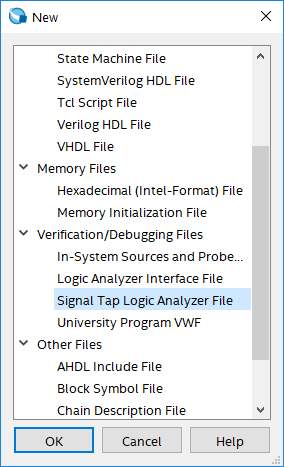
\includegraphics[scale=0.65]{figures/figure3.png}
   \caption{Need to prepare a new file.} 
	 \label{fig:3}
	 \end{center}
\end{figure}

\item The SignalTap window with the {\sf Setup} tab selected is depicted in Figure~\ref{fig:4}. Save the file under
the name {\it keys.stp}. In the dialog
box that follows (Figure~\ref{fig:5}), click {\sf OK}. For the dialog "Do you want to enable SignalTap file
'keys.stp' for the current project?" click {\sf Yes} (Figure~\ref{fig:6}). The file {\it keys.stp} is now the SignalTap 
file associated with the project. 

Note: If you want to disable this file from the project, or to disable SignalTap from the project, 
go to {\sf Assignments > Settings}. In the category list, select {\sf SignalTap Logic Analyzer}, bringing up the
window in Figure~\ref{fig:7}. To turn off the analyzer, uncheck {\sf Enable SignalTap Logic Analyzer}.
It is possible to have multiple SignalTap files for a given project, but only one of them can
be enabled at a time. Having multiple SignalTap files might be useful if the project is very large and different
sections of the project need to be probed. To create a new SignalTap file for a project, simply follow
Steps 1 and 2 again and give the new file a different name. To change the SignalTap file associated with the project, in the {\sf SignalTap File
name} box browse for the file wanted, click {\sf Open}, and then click {\sf OK}.  For this tutorial we want to leave SignalTap enabled and we want 
the SignalTap File name to be {\it keys.stp}. Make sure this is the case and click {\sf OK} to leave the settings window. 
  
\begin{figure}[H]
   \begin{center}
      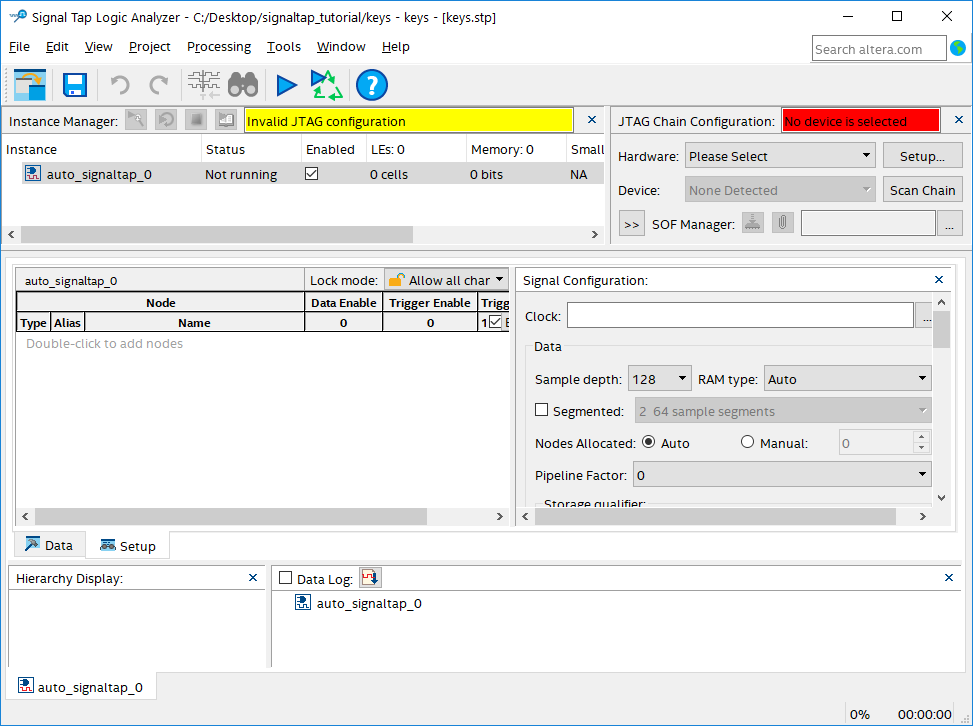
\includegraphics[scale=0.6]{figures/figure4.png}
   \caption{The SignalTap window.} 
	 \label{fig:4}
	 \end{center}
\end{figure}

\begin{figure}[H]
   \begin{center}
      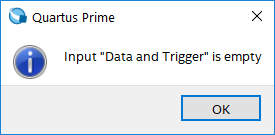
\includegraphics[scale=0.65]{figures/figure5.png}
   \caption{Click {\sf OK} to this dialog.} 
	 \label{fig:5}
	 \end{center}
\end{figure}

\begin{figure}[H]
   \begin{center}
      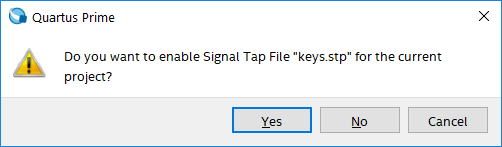
\includegraphics[scale=0.65]{figures/figure6.png}
   \caption{Click {\sf Yes} to this dialog.} 
	 \label{fig:6}
	 \end{center}
\end{figure}

\begin{figure}[H]
   \begin{center}
      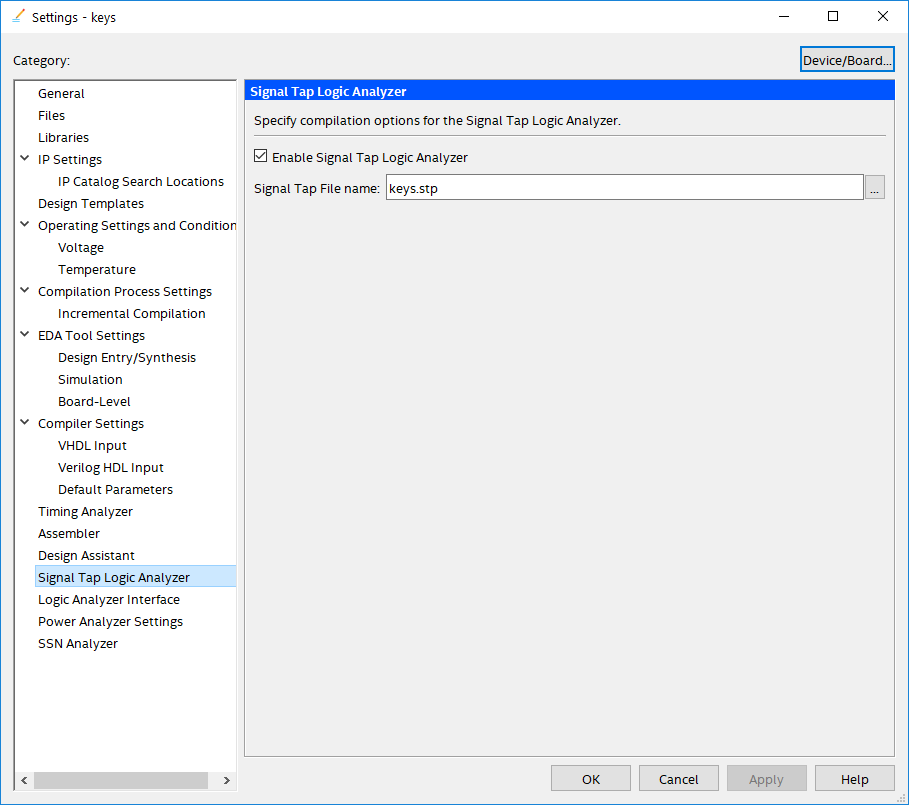
\includegraphics[scale=0.6]{figures/figure7.png}
   \caption{The SignalTap Settings window.} 
	 \label{fig:7}
	 \end{center}
\end{figure}

\item We now need to add the nodes in the project that we wish to probe. In the Setup tab of the SignalTap window, double-click
in the area labeled  {\sf Double-click to add nodes}, bringing up the Node Finder window 
shown in Figure~\ref{fig:8}. Click on 
\includegraphics[scale=0.7]{figures/icon3.png} or 
\includegraphics[scale=0.7]{figures/icon6.png} to show or hide more search options. 
For the {\sf Filter} field, select {\sf SignalTap: pre-synthesis}, and
for the {\sf Look in} field select {\sf |keys|}.
Click {\sf List}. This will now display all the nodes that can be probed in the project. 
Highlight KEY[0] to KEY[3], and then click the 
\includegraphics[scale=0.90]{figures/icon4.png} button to add the keys to be probed.
Click {\sf Insert} to insert the selected nodes, then {\sf Close} to close the Node Finder window.

\begin{figure}[H]
   \begin{center}
      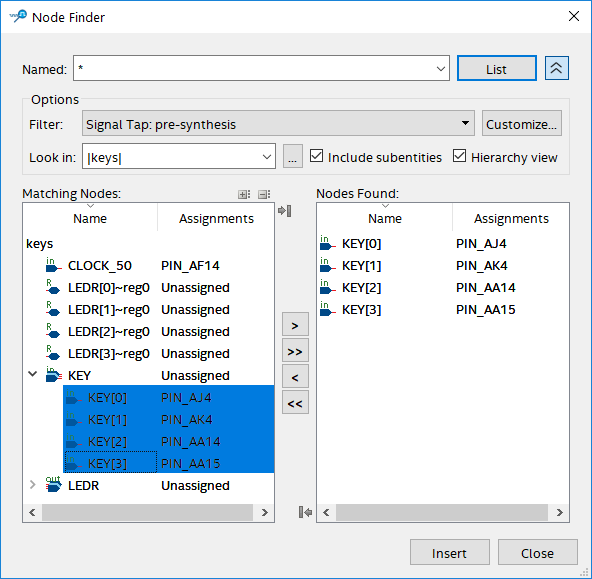
\includegraphics[scale=0.6]{figures/figure8.png}
   \caption{Adding nodes in the Node Finder window on a DE-series board.} 
	 \label{fig:8}
	 \end{center}
\end{figure}

\item Before the SignalTap analyzer can work, we need to specify what clock is going
to run the SignalTap module that will be instantiated within our design. To do this, in the Clock box of the
Signal Configuration pane of the SignalTap window, click 
\includegraphics[scale=0.7]{figures/icon5.png}, which will again bring up the Node Finder window.
Select {\sf List} to display all the nodes that can be added as the clock, and then double-click CLOCK\_50, which
results in the image shown in Figure~\ref{fig:9}. Click {\sf OK}.
  
\begin{figure}[H]
   \begin{center}
      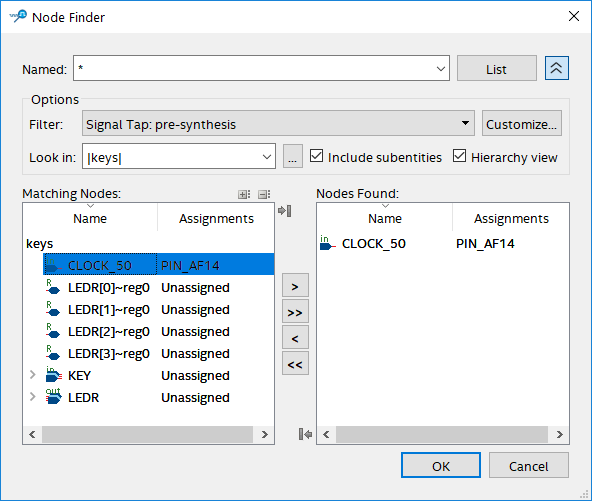
\includegraphics[scale=0.6]{figures/figure9.png}
   \caption{Setting CLOCK\_50 as the clock for the SignalTap instance on a DE-series board.} 
	 \label{fig:9}
	 \end{center}
\end{figure}

\item With the {\sf Setup} tab of the SignalTap window selected, select the checkbox in the Trigger Conditions column. In the dropdown
menu at the top of this column, select {\sf Basic AND}. Right-click on the Trigger Conditions cell corresponding to the node 
KEY[0] and select {\sf Low}. Now, the trigger for running the Logic Analyzer will be when the first key on the DE-series board
is pressed, as shown in Figure~\ref{fig:10}.
Note that you can right-click on the Trigger Conditions cell of any of the nodes being probed and select the trigger
condition from a number of choices. The actual trigger condition will be true when the logical AND of all these
conditions is satisfied. For now, just keep the trigger condition as KEY[0] set to low and the others set to their default value, 
{\sf Don't Care}.
  
\begin{figure}[H]
   \begin{center}
      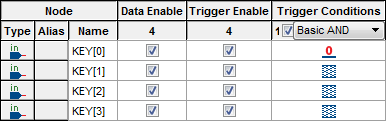
\includegraphics[scale=0.6]{figures/figure10.png}
   \caption{Setting the trigger conditions.} 
	 \label{fig:10}
	 \end{center}
\end{figure}

\item For SignalTap to work, we need to properly set up the hardware. First, make sure the DE-series
board is plugged in and turned on. In the Hardware section
of the SignalTap window, located in the top right corner, click {\sf Setup...}, bringing up the window
in Figure~\ref{fig:11}. Double click DE-SoC in the Available Hardware Items menu, then click {\sf Close}.
If you are using a DE0-CV, DE0-Nano, DE2-115, or the DE10-Lite, you will select USB-Blaster from the Available Hardware Items menu.
  
\begin{figure}[H]
   \begin{center}
      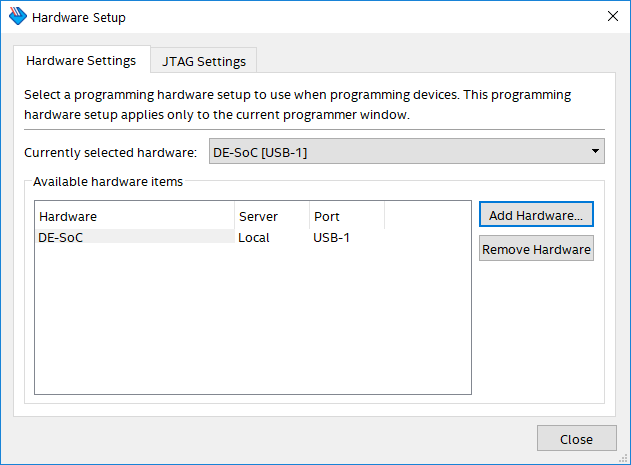
\includegraphics[scale=0.6]{figures/figure11.png}
   \caption{Setting up hardware.} 
	 \label{fig:11}
	 \end{center}
\end{figure}

\item In the Device section of the main SignalTap window, select the device that corresponds to the FPGA on your DE-series board.
Do not select the {\sf SOCVHPS} device as this corresponds to the ARM Cortex-A9* processor.
If you are using the DE0-CV, DE0-Nano, DE2-115, or DE10-Lite there should be only one device that is selectable.
\item The last step in instantiating SignalTap in your design is to compile the design. In the main Quartus Prime window,
select {\sf Processing > Start Compilation} and indicate that you want to save the changes to the file by clicking {\sf Yes}.
After compilation, go to {\sf Tools > Programmer} and load
the project onto the DE-series board. You may also need to select the corresponding SOF file in the SOF Manager box in the main SignalTap window.
\end{enumerate}

\section{Probing the Design Using SignalTap}

Now that the project with SignalTap instantiated has been loaded onto the DE-series board, we can
probe the nodes as we would with an external logic analyzer.

\begin{enumerate}

\item On the DE-series board, first ensure that none of the keys (0-3) is being pressed. We will try to probe the values of these keys once key 0 is pressed.

\item In the SignalTap window, select {\sf Processing > Run Analysis} or click the 
\includegraphics[scale=0.7]{figures/icon1.png} icon. You should get a screen similar to Figure~\ref{fig:12}. Note that the status column of the SignalTap Instance Manager pane says "Waiting for
trigger." This is because the trigger condition (Key 0 being low) has not yet been met.
  
\begin{figure}[H]
   \begin{center}
      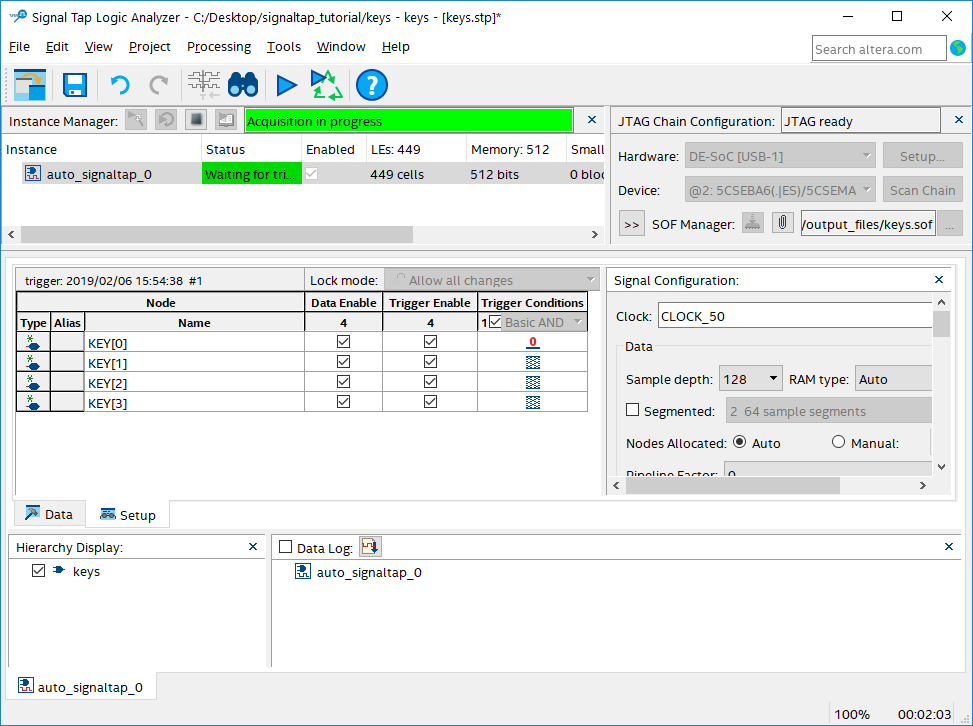
\includegraphics[scale=0.65]{figures/figure12.png}
   \caption{SignalTap window on a DE-series board after Run Analysis has been clicked.} 
	 \label{fig:12}
	 \end{center}
\end{figure}

\item Now, to observe the trigger feature of the Logic Analyzer, click
on the {\sf Data} tab of the SignalTap Window and then press and hold Key 0 on the DE-series board. The data window
of the SignalTap window should display the image in Figure~\ref{fig:13}. Note that this window shows the data levels
of the 4 nodes before and after the trigger condition was met. As an exercise, unpress Key 0 then click {\sf Run Analysis} again. Hold down any of Keys 1-3, then press Key 0. When Key 0 is pressed, you will see that the values of Keys 1-3
displayed on the SignalTap Logic Analyzer match what is being pressed on the board.
  
\end{enumerate}

\begin{figure}[H]
   \begin{center}
      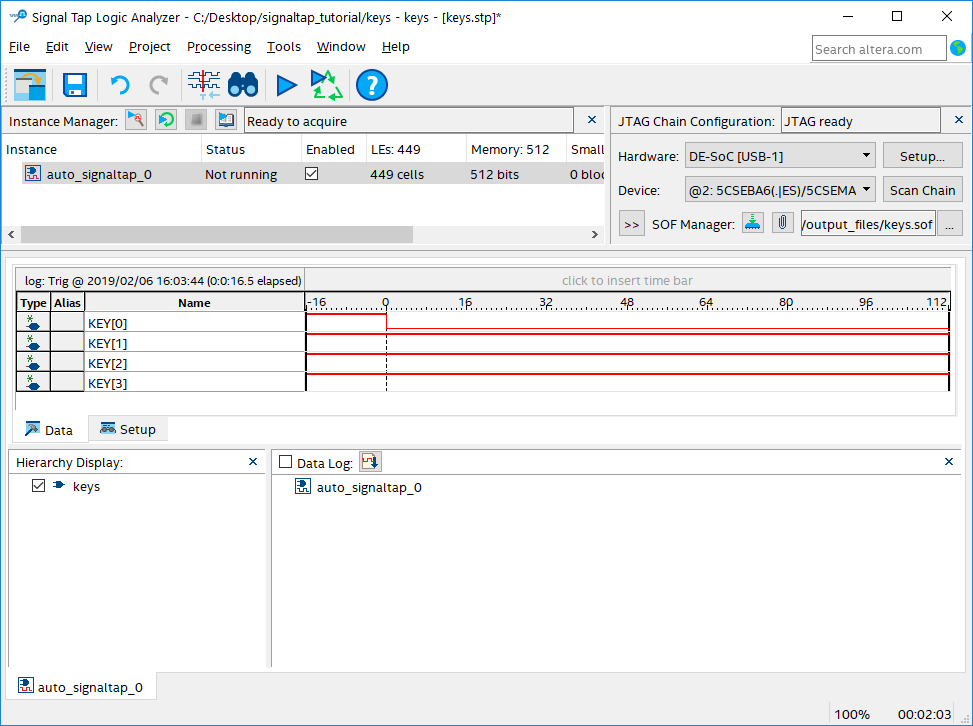
\includegraphics[scale=0.65]{figures/figure13.png}
   \caption{Graphical display of values after trigger condition is met.} 
	 \label{fig:13}
	 \end{center}
\end{figure}

\section{Advanced Trigger Options}
Sometimes in a design you may want to have a more complicated triggering condition than SignalTap's basic
triggering controls allow. The following section describes how to have multiple trigger levels.
% as well as how to create advanced triggering options.

\subsection{Multiple Trigger Levels}

In this section, we will set up the analyzer to trigger when there is a positive edge from Key 0, Key 1,
Key 2, and then Key 3, in that order.
\begin{enumerate}
\item Click the {\sf Setup} tab of the SignalTap window.
  
\item In the Signal Configuration pane, select 4 from Trigger Conditions dropdown menu as in Figure~\ref{fig:14} (you may have to scroll down in the Signal Configuration pane to see this menu). This modifies the node list
window by creating three new Trigger Conditions columns.
  
\begin{figure}[H]
   \begin{center}
      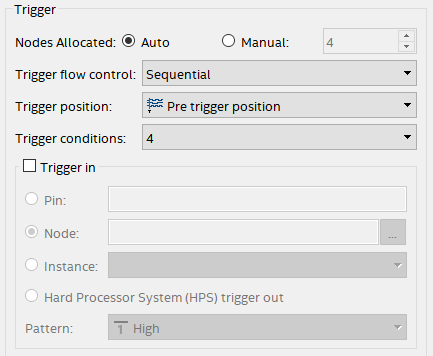
\includegraphics[scale=0.65]{figures/figure14.png}
   \caption{Set trigger conditions to 4.} 
	 \label{fig:14}
	 \end{center}
\end{figure}

\item Right click the Trigger Condition 1 cell for KEY[0], and select {\sf Rising Edge}. Do the same for the Trigger Condition 2 cell
for KEY[1], Trigger Condition 3 for KEY[2], and Trigger Condition 4 for KEY[3]. You should end up with a window that looks
like Figure~\ref{fig:15}.

\begin{figure}[H]
   \begin{center}
      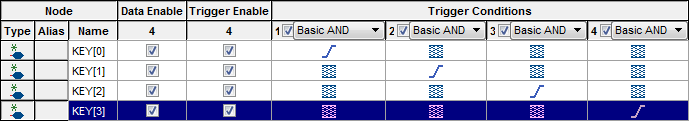
\includegraphics[scale=0.65]{figures/figure15.png}
   \caption{Multiple trigger levels set.} 
	 \label{fig:15}
	 \end{center}
\end{figure}

\item Now, recompile the design and load it onto the DE-series board again.
  
\item Go back to the SignalTap window, click on the Data tab, and then click {\sf Processing > Run Analysis}. Note that the window
will say "Waiting for trigger" until the appropriate trigger condition is met. Then, in sequence, press and release keys 0, 1, 2, and then 3.

After this has been done, you will see the values of all the keys displayed as in Figure~\ref{fig:16}. Experiment by following
the procedure outlined in this section to set up other trigger conditions and use the DE-series board to test these trigger
conditions.

If you want to continuously probe the analyzer, instead of clicking "Run Analysis,"  click "Autorun Analysis" which
is the icon right next to the "Run Analysis" icon. If you do this, every time the trigger condition is met the value in the
display will be updated. You do not have to re-select "Run Analysis." To stop the "Autorun Analysis" function, click the 
\includegraphics[scale=0.7]{figures/icon2.png} icon.
  
\begin{figure}[H]
   \begin{center}
      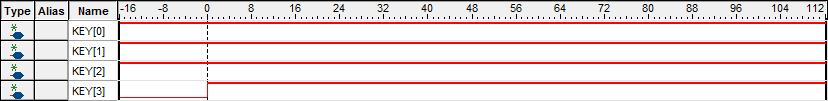
\includegraphics[scale=0.65]{figures/figure16.png}
   \caption{Logic Analyzer display when all four trigger conditions have been met.} 
	 \label{fig:16}
	 \end{center}
\end{figure}

\end{enumerate}

\subsection{Advanced Trigger Conditions}
In this section we will learn how to create advanced trigger conditions. Our trigger condition will
be whenever any one of the first 3 LED displays  have a positive or negative edge. This means that the Logic Analyzer will
update its display every time one of these inputs changes. Note that we could have any logical function of the nodes being
probed to trigger the analyzer. This is just an example. After you implement this in the next few steps, experiment
with your own advanced triggers. 
\begin{enumerate}
\item Have the {\it keys} project opened and compiled from the previous examples in this tutorial.
  
\item Open the SignalTap window and select the Setup tab. In the Signal Configuration pane make sure that the number
of Trigger Conditions is set to 1.
  
\item In the Trigger Conditions column of the node list, make sure the box is checked and select {\sf Advanced} from the dropdown
menu as in Figure~\ref{fig:17}. This will immediately bring up the window in Figure~\ref{fig:18}. This window allows you to create a logic circuit using
the various nodes that you are probing with SignalTap.
  
\begin{figure}[H]
   \begin{center}
      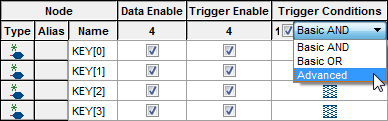
\includegraphics[scale=0.65]{figures/figure17.png}
   \caption{Select Advanced from the Trigger Level dropdown menu.} 
	 \label{fig:17}
	 \end{center}
\end{figure}

\begin{figure}[H]
   \begin{center}
      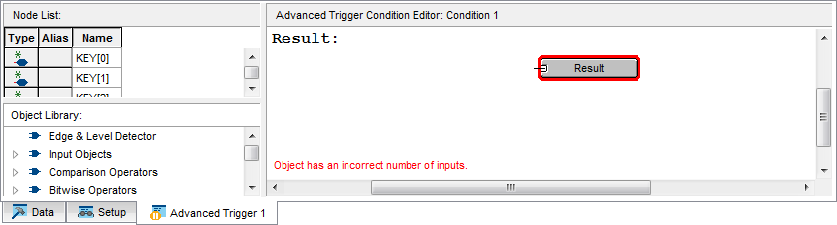
\includegraphics[scale=0.65]{figures/figure18.png}
   \caption{The Advanced Trigger editing window.} 
	 \label{fig:18}
	 \end{center}
\end{figure}

\item In the node list section of this window, highlight the 3 nodes KEY[0] to KEY[2], and click and drag them into the white space
of the Advanced trigger window, resulting in Figure~\ref{fig:19}. Note that you can also drag and drop each node individually.
  
\begin{figure}[H]
   \begin{center}
      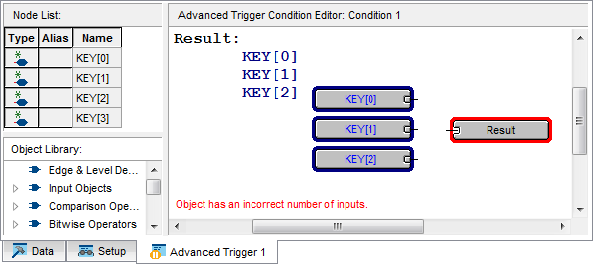
\includegraphics[scale=0.65]{figures/figure19.png}
   \caption{The three input nodes of interest dragged into the Advanced Trigger Editing Window.} 
	 \label{fig:19}
	 \end{center}
\end{figure}

\item We now need to add the necessary logical operators to our circuit. We will need an OR gate as well as three edge level detectors. To access
the OR gate, expand {\sf Logical Operators} in the Object Library and select {\sf Logical Or}, as in Figure~\ref{fig:20}. Then drag and drop
the operator into the editing window.
  
\begin{figure}[H]
   \begin{center}
      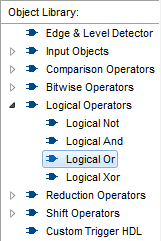
\includegraphics[scale=0.65]{figures/figure20.png}
   \caption{Select the Logical Or operator from the Object Library window and drag this into the editing window.} 
	 \label{fig:20}
	 \end{center}
\end{figure}

\item In the object library click {\sf Edge and Level Detector} and drag this into the editing window. Do this three times and then arrange
the circuit as in Figure~\ref{fig:21}. The three inputs should each be connected to the input of an edge and level detector and the 
output of each of these detectors should be connected to the OR gate. The output of the OR gate should 
be connected to the output pin already in the editing window.
  
\begin{figure}[H]
   \begin{center}
      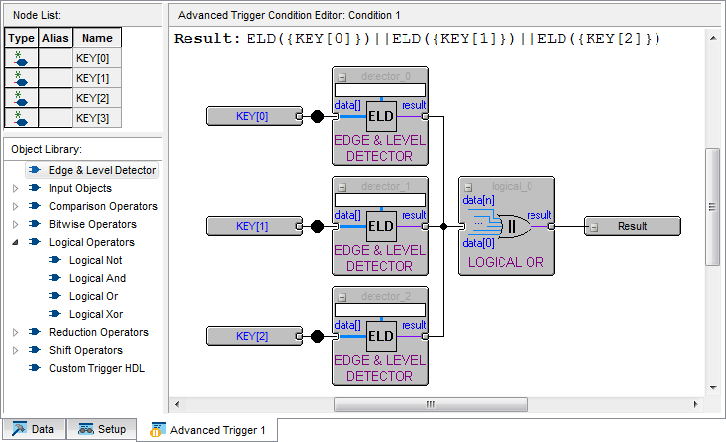
\includegraphics[scale=0.65]{figures/figure21.png}
   \caption{Arrange the elements to create a circuit that looks like this.} 
	 \label{fig:21}
	 \end{center}
\end{figure}

\item We now need to set each edge and level detector to sense either a falling edge or a rising edge. 
Double click one of the edge and level detectors,
bringing up the window in Figure~\ref{fig:22}. Type E in the setting box and then click {\sf OK}. This will mean that the detector will output 1 whenever
there is either a falling edge or a rising edge of its input. Repeat this step for the two remaining edge and level detectors.

\begin{figure}[H]
   \begin{center}
      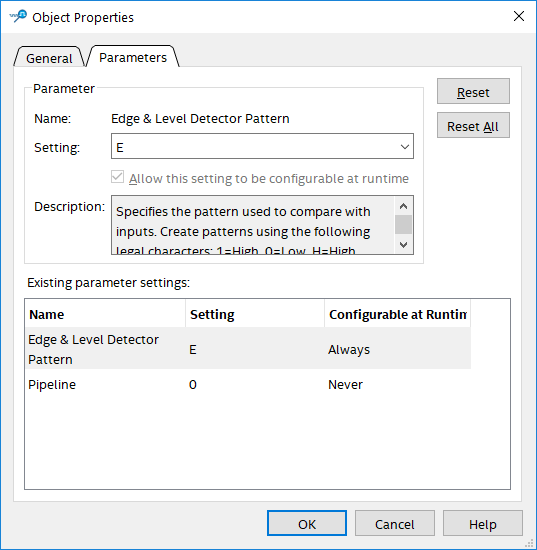
\includegraphics[scale=0.60]{figures/figure22.png}
   \caption{Type E in the setting box so that the function triggers on both rising and falling edges.} 
	 \label{fig:22}
	 \end{center}
\end{figure}

\item To test this Advanced trigger condition, compile the designed circuit again and load it onto the DE-series board. Then run Signal Tap as 
described in the previous section. You should note that the Analyzer should sense every time you change one of the first
three keys on the board.
  
\end{enumerate}

\section{Sample Depth and Buffer Acquisition Modes}
In this section, we will learn how to set the Sample Depth of our analyzer and about the two buffer acquisition modes.
To do this, we will use the previous project and use segmented buffering. Segmented buffering allows us to divide the acquisition
buffer into a number of separate, evenly sized segments. We will create a sample depth of 128 bits and divide this into
eight 32-sample segments. This will allow us to capture 4 distinct events that occur around the time of our trigger.
\begin{enumerate}
\item Change the trigger condition back to Basic AND and have only one trigger condition.
Make the trigger condition to be at the falling edge of KEY[0].
  
\item In the Signal Configuration pane of the SignalTap window, in the {\sf Sample depth} dropdown menu of the Data pane select {\sf 128}. This option allows you to specify how many samples will be taken around the triggers
in your design. If you require many samples to debug your design, select a larger sample depth. Note, however, that if
the sample depth selected is too large, there might not be enough room on the board to hold your design
and the design will not compile. If this happens, try reducing the sample depth.
  
\item In the Signal Configuration pane of the SignalTap window, in the Data section of the pane check {\sf Segmented}.
In the dropdown menu beside Segmented, select {\sf 4 32 sample segments}. This will result in a pane that looks like
Figure~\ref{fig:23}.
  
\begin{figure}[H]
   \begin{center}
      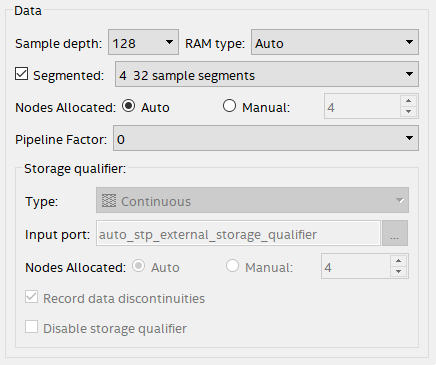
\includegraphics[scale=0.65]{figures/figure23.png}
   \caption{Select Segmented buffer acquisition mode with 4 32 sample segments.} 
	 \label{fig:23}
	 \end{center}
\end{figure}

\item Recompile and load the designed circuit onto the DE-series board. Now, we will be able to probe the design
using the Segmented Acquisition mode.
  
\item Go back to the SignalTap window and click {\sf Processing > Run Analysis}. Now, press and release KEY[0], and in between clicks
change the values of the other 3 keys. After you have done this 4 times, the values
in the buffer will be displayed in the data window, and this will display the values that the 4 keys had at around each trigger.
A possible waveform is presented in Figure~\ref{fig:24}. This resulted from the user pressing and holding one more key between each click of KEY[0].
  
\end{enumerate}

\begin{figure}[H]
   \begin{center}
      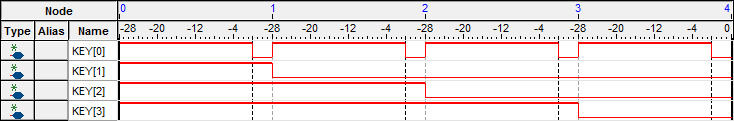
\includegraphics[scale=0.65]{figures/figure24.png}
   \caption{Possible waveforms that could result when using the Segmented Acquisition mode.} 
	 \label{fig:24}
	 \end{center}
\end{figure}

\subsection{Use of Synthesis Keep Directive}

Sometimes a design you create will have wires in it that the Quartus compiler will optimize away. A very simple example
is the Verilog code below:

% \begin{figure}[H]
% \begin{center} %%%\begin{singlespace}
% \parbox{12.5cm}{
% \begin{tabbing}
% ZZ\=ZZ\=ZZ\=ZZ\=ZZ\=ZZ\kill
% {\bf module} threeInputAnd(SW, LEDR, CLOCK\_50);\\
% \>{\bf input} CLOCK\_50;\\
% \>{\bf input} [2:0] SW;\\
% \>{\bf output reg} [0:0] LEDR;\\
% \\
% \>{\bf wire} ab, abc /*synthesis keep*/;\\
% \\
% \>{\bf assign} ab=SW[0]\&SW[1];\\
% \>{\bf assign} abc=ab\&SW[2];\\
% \\
% \>{\bf always} @ (posedge CLOCK\_50)\\
% \>{\bf begin}\\
% \>\>\>  LEDR[0]<=abc;\\
% \>{\bf end}\\

% {\bf endmodule}\\
% \end{tabbing} }
	% \caption{Using the Synthesis Keep directive in Quartus Prime.}
	% \label{fig:25}
% \end{center}
% \end{figure}

\begin{figure}[H]
\begin{lstlisting}[language=Verilog, xleftmargin=.3\textwidth]
module threeInputAnd(SW, LEDR, CLOCK_50);
	input CLOCK_50;
	input [2:0] SW;
	output reg [0:0] LEDR;

	wire ab, abc /*synthesis keep*/;

	assign ab=SW[0]&SW[1];
	assign abc=ab&SW[2];
	
	always @ (posedge CLOCK_50)
	begin
		LEDR[0]<=abc;
	end
endmodule

\end{lstlisting}
     \caption{Using the Synthesis Keep directive in Quartus Prime.}
	 \label{fig:25}
\end{figure}
 
A diagram of this circuit is shown in Figure~\ref{fig:26}. The triangular symbols labeled
{\bf ab} and {\bf abc} are buffers inserted by Quartus. They do not modify the
signals passing through them.

\begin{figure}[H]
   \begin{center}
      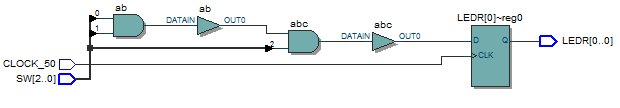
\includegraphics[scale=0.65]{figures/figure26.png}
   \caption{The circuit implemented by the code in Figure~\ref{fig:25}} 
	 \label{fig:26}
	 \end{center}
\end{figure}

We wish to instantiate a SignalTap module that will probe the values of the inputs SW[2:0] and the outputs LEDR[2:0]. We also want to
probe the internal wire {\bf ab}. However, normally when this Verilog code is compiled (without the /*synthesis keep*/ directive), the wire {\bf ab} is optimized away into one logic element, as in Figure~\ref{fig:27}.

\begin{figure}[H]
   \begin{center}
      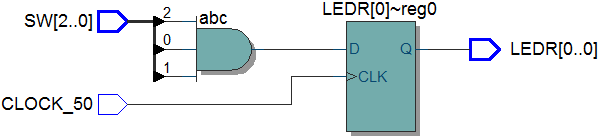
\includegraphics[scale=0.65]{figures/figure27.png}
   \caption{The same circuit without the Synthesis Keep directive.} 
	 \label{fig:27}
	 \end{center}
\end{figure}

If you wish to probe this internal wire, however, you will have to direct Quartus that you do not want this wire to be optimized away.
To do so, place the text {\it /*synthesis keep*/} on the line that declares the wire, right before the semicolon of the line.
Figure~\ref{fig:25} already contains this directive. We will now demonstrate how this wire can be probed:

\begin{enumerate}
\item Create a new Quartus project threeInputAnd and copy the Verilog code from Figure~\ref{fig:25}. Compile the project.
\item Go to {\sf Tools > SignalTap Logic Analyzer}, and then in the Setup pane of the SignalTap window, right click
and choose {\sf Add Nodes}.
\item For the {\sf Filter} field, select {\sf SignalTap: pre-synthesis}. Select {\sf |threeInputAnd|} in the {\sf Look in} drop-down menu and click the {\sf List} button. Move the nodes {\bf ab}, {\bf SW[0]}, {\bf SW[1]}, {\bf SW[2]}, and {\bf LEDR[0]} into the Selected Nodes list and then click {\sf OK}.
\item In the Signal Configuration pane, select {\bf CLOCK\_50} as the clock signal.
\item Set a Trigger Condition to trigger when {\bf ab} becomes high.
\item Import the relevant pin assignment file for the DE-series board (or assign the pins manually, as described in Section 7 of the Quartus Prime Introduction tutorials). For a DE1-SoC board, this file is named {\it DE1\_SoC.qsf}
\item Compile the project again.
\item Go to {\sf Tools > Programmer} and load the circuit onto the DE-series board.
\item Open the SignalTap window again, and select the Data tab. Set all the switches on the DE-series board to the low position. Then, start the analysis by selecting {\sf Processing > Run Analysis}.
\item Set the first two switches to the high position. The Trigger Condition should be satisfied.
\end{enumerate}


% Copyright and Trademark

%\newcommand{\datePublished}{Mar 2022}

\newcommand{\versnum}{21.1} %version number quartus/AMP
\newcommand{\quartusname}{Quartus\textsuperscript{\textregistered} Prime}	
\newcommand{\textBar}{For \quartusname{} \versnum{}}
\newcommand{\thisyear}{2022 } %for copyright
\newcommand{\company}{FPGAcademy.org}
\newcommand{\longteamname}{FPGAcademy.org}
\newcommand{\teamname}{FPGAcademy}
\newcommand{\website}{FPGAcademy.org}

\newcommand{\productAcronym}{AMP}
\newcommand{\productNameShort}{Monitor Program}

\newcommand{\productNameMedTM}{Monitor Program}
\newcommand{\productNameMed}{Monitor Program}

%\newcommand{\headerLogoFilePath}[1]{#1/FPGAcademy.png}



%%%%%%%%%%%%%%%%%%%%%%%%%%%%%%%%%%%%%%%%
%%% FPGAcademy Copyright Information %%%
%%%%%%%%%%%%%%%%%%%%%%%%%%%%%%%%%%%%%%%%

%Always put the copyright on a new page (clear page), with some vertical space from top
\clearpage
\vspace{1in}

\noindent

Copyright {\copyright} FPGAcademy.org. All rights reserved. FPGAcademy and the FPGAcademy logo are trademarks of  FPGAcademy.org.  This document is being provided on an ``as-is'' basis and as an accommodation and therefore all warranties, representations or guarantees of any kind (whether express, implied or statutory) including, without limitation, warranties of merchantability, non-infringement, or fitness for a particular purpose, are specifically disclaimed.

%FPGAcademy assumes no responsibility or liability arising out of the application or use of any information,  product,  or  service  described  herein  except  as  expressly  agreed  to  in  writing  by  FPGAcademy.



**Other names and brands may be claimed as the property of others.




\end{document}
